\documentclass[twocolumn]{article}

\usepackage[utf8]{inputenc}
\usepackage[T1]{fontenc}
\usepackage{amsmath,amssymb,amsfonts}
\usepackage{booktabs}
\usepackage{graphicx}
\usepackage{hyperref}
\usepackage{xcolor}
\usepackage{algorithm}
\usepackage{algorithmic}
\usepackage{geometry}
\usepackage{enumitem}
\usepackage{subcaption}
\usepackage{natbib}
\usepackage{tikz}
\usepackage{pgfplots}
\pgfplotsset{compat=1.18}

\geometry{margin=0.75in}

\newcommand{\R}{\mathbb{R}}
\newcommand{\N}{\mathbb{N}}
\newcommand{\EE}{\mathcal{E}}
\newcommand{\DD}{\mathcal{D}}
\newcommand{\MM}{\mathcal{M}}
\newcommand{\CC}{\mathcal{C}}
\newcommand{\DCI}{DCI}
\newcommand{\bx}{\mathbf{x}}
\newcommand{\bw}{\mathbf{w}}
\newcommand{\bs}{\mathbf{s}}

\title{Behavioral Signatures of Deliberation:\\A Deterministic Model of Drive-Conflict Resolution}

\author{Zierax}
\date{2026}

\begin{document}

\maketitle

\begin{abstract}
We present AXIOM-02, a deterministic simulation engine that models high-stakes
cognitive dissonance and drive-conflict resolution in narrative scenarios drawn
from canonical works of literature and philosophy. Unlike reward-maximising
agents that resolve choices via argmax, AXIOM-02 employs a mutual inhibition
network of 18 affective drives modulated by 5 neuromodulatory systems, producing
behavioural signatures such as deadlock, spite-driven rejection of rational
optima, and moral residue bleed across sequential dilemmas. We introduce a
weighted composite deliberative complexity metric,
$\DCI = \sum_{i=1}^{8} w_i \cdot C_i$, over eight criteria: status-differential
sensitivity, transition oscillation, irrationality signal, betrayal-cascade
amplification, deadlock frequency, spite index, moral-residue bleed, and
paradoxical attachment. Across 102 scenarios---including Dostoevsky's
Underground Man, Sophie's Choice, and the trolley problem---the engine's
chosen action matches the documented human expected action in 66.7\% of
scenarios, versus 33.3\% (argmax) and 28.4\% (random; chance
$\approx 24\%$). Measured ablation shows the composite is dominated by
the single binary criterion C3 (irrationality; $\rho = 0.944$, $R^2 =
0.891$), so the composite is reported as a diagnostic, not a validated
measure of complexity; C1 is inactive in suite runs and C7 is saturated
by the shared residue state. Verdict labels are shown to be
seed-dependent (53--71 COMPLEX across seeds) despite per-seed
determinism. This work targets the inhibition-deliberation thesis as a
testable hypothesis about the structure of conflicted decision
processes, not as a claim about consciousness.
\end{abstract}

% ============================================================================
\section{Introduction}
\label{sec:introduction}

The measurement of deliberation in computational systems remains an open
problem in cognitive science. Classical decision-theoretic agents resolve
conflicts by maximising expected utility, producing choices that are
deterministic given complete information---yet human deliberation is
characterised precisely by its resistance to such resolution. When faced
with moral dilemmas, humans exhibit prolonged indecision, oscillation
between competing values, and---critically---occasionally choose options
that are demonstrably worse for themselves \citep{dostoevsky1864}.

This paper addresses the question: \emph{Can a deterministic computational
system produce behavioural signatures that relate to human
intuitions about deliberative depth?} We approach this not through neural simulation
but through a carefully engineered drive-conflict architecture that
replicates the phenomenology of moral struggle.

The contribution is threefold. First, we formalise a mutual inhibition
network in which drives suppress each other asymmetrically, producing
effective activations that differ qualitatively from raw activations
(Section~\ref{sec:framework}). Second, we define eight measurable
deliberative criteria---from deadlock frequency to moral-residue bleed---
and combine them into a composite metric $\DCI$ (Section~\ref{sec:probe}).
Third, we evaluate the system against 102 scenarios drawn from canonical
literature, reporting measured action fidelity and an honest
characterisation of $\DCI$'s limitations (Section~\ref{sec:experiments}).

% ============================================================================
\section{Related Work}
\label{sec:related}

\subsection{Computational Models of Emotion}

The \citet{ortony1988} (OCC) model remains the most influential cognitive
appraisal theory, structuring emotions as consequences of evaluations along
three dimensions: valence of outcome (pleasant/unpleasant), agency
(self/other), and circumstances (situation/event). Each of the 22 emotion
types is derived from a binary decision tree, making OCC fully computable
\citep{gratch2014}. OCC generates \emph{discrete emotion labels} from
appraisal variables---a single evaluation pathway yields a single,
unambiguous emotion type. AXIOM-02 departs fundamentally: its 18 drives
are not discrete emotion labels but \emph{motivational states} with
continuous activation and mutual inhibition. Crucially, AXIOM-02's
inter-drive suppression produces emergent deliberative
signatures---deadlock oscillation, spite-driven rejection of rational
optima, and moral residue bleed across sequential dilemmas---that OCC's
tree structure cannot generate, because each appraisal yields a single
outcome with no mechanism for sustained inter-drive competition.

BDI (Belief-Desire-Intention) architectures \citep{bratman1987,
rao1995} model agents as rational deliberators that maintain explicit
beliefs about the world, desires that motivate action, and intentions
that commit resources to plans. BDI systems are well-suited to
goal-directed behaviour but treat conflict resolution as a planning
problem---agents select intentions via pragmatic reasoning rather than
emotional competition. AXIOM-02 has no explicit beliefs or goals; drives
compete directly through mutual inhibition, producing deliberative
signatures without propositional representation. The deadlock state---
in which no single drive dominates---is a state that BDI architectures
explicitly avoid by design. Marsella and Gratch's EMA model
\citep{marsella2009} extended BDI with appraisal dynamics, demonstrating
that emotions emerge from agent-environment interaction loops. While EMA
captures appraisal \emph{processes}, AXIOM-02 focuses on the
\emph{behavioural signatures} of post-appraisal drive conflict: what
happens when multiple appraisals are simultaneously valid and mutually
contradictory.

\subsection{Consciousness Measures}

Integrated Information Theory \citep{tononi2004} proposes that
consciousness corresponds to a system's capacity to integrate information,
quantified by $\Phi$. AXIOM-02's DCI is explicitly \emph{not} IIT's
$\Phi$---this distinction is critical. Where $\Phi$ measures integration
across \emph{all} system states (capturing the \emph{capacity} for
experience), DCI measures specific behavioural correlates of
deliberative struggle (capturing the \emph{behavioural signature} of
conflicted agency). A system may have high $\Phi$ yet produce no deadlock
(if drives are additive rather than inhibitory), or high DCI with modest
$\Phi$ (if inhibition is concentrated among a few drives). The two metrics
are complementary rather than competing: $\Phi$ addresses the hard problem
of phenomenal experience, while DCI operationalises the softer but more
empirically tractable question of deliberative depth.

Global Workspace Theory \citep{baars1988} models consciousness as a
broadcast mechanism whereby information selected by a limited-capacity
workspace is made available to specialist processors. In GWT, the
workspace functions as a bottleneck: only one coalition of representations
gains access at a time, and competition among coalitions determines which
representation is broadcast. AXIOM-02's deadlock mechanism resembles GWT
competition, but operates on \emph{affective drives} rather than cognitive
representations. When no coalition of drives satisfies both the fire
threshold $\tau_f$ and the margin $\tau_s$, the workspace effectively
broadcasts \emph{nothing}, producing the system-level hesitation that
correlates with deliberative depth. This is structurally analogous to GWT's
competition phase, but the competing items are motivational states with
mutual inhibition rather than propositional contents.

Higher-Order Theories of consciousness \citep{rosenthal2005} propose that
a mental state is conscious only when it is the object of a
higher-order representation---that is, consciousness requires
self-monitoring of one's own mental states. AXIOM-02's
MetaCognitiveMonitor implements a \emph{structural analog} of this
mechanism: it detects and reports deadlock by monitoring the drive
activation landscape, performing a functionally analogous role to
higher-order representation. However, AXIOM-02 does not attribute
phenomenal consciousness to the system. The meta-cognitive layer is a
diagnostic mechanism that enables the deliberative probe to detect
hesitation, not a claim about the system's subjective experience.

\subsection{Moral Reasoning in AI}

The Moral Machine experiment \citep{awad2018} collected 40 million
ethical decisions from participants across 233 countries, revealing
systematic cultural variation in trolley-type judgements. While the
Moral Machine paradigm elicits \emph{individual} moral preferences,
AXIOM-02 models the \emph{internal conflict} that produces those
preferences. In Awad et al.'s paradigm, the agent chooses; in AXIOM-02's
paradigm, the agent's internal state \emph{oscillates} before choosing.
AXIOM-02 uses literary scenarios as moral test cases, producing
deliberative complexity scores (DCI) whose limitations we characterise
in Section~\ref{sec:results}. The moral-residue bleed mechanism (C7)
extends this further: prior moral choices contaminate future
deliberation, producing path-dependent trace dynamics that
cross-sectional moral-judgement studies cannot capture.

The trolley problem \citep{thomson1985} and its variants have become
the canonical stimulus for studying moral judgement. Greene et al.'s
fMRI studies \citep{greene2001} showed that personal moral dilemmas
(those requiring direct physical contact with the victim) activate
emotional brain regions including the ventromedial prefrontal cortex and
amygdala, whereas impersonal dilemmas (such as diverting a trolley)
engage dorsolateral prefrontal areas associated with deliberative
reasoning. AXIOM-02 is \emph{inspired by} this dissociation as a design
metaphor: the mutual inhibition network produces emotional oscillation
and deadlock when affective drives (empathy, grief, rage) compete with
cold logic in a single (non-dual-process) network. We do not claim to
replicate any neural activation pattern or neurological finding; the
parallel is architectural and metaphorical. The irrationality signal
(C3)---measuring deviation from the cold baseline toward love- or
sacrifice-biased responses---is a proxy for the idea of emotional
override, and the mechanism is explicitly non-modular.

\subsection{Affective Computing}

\citet{picard1997} established affective computing as a field, arguing
that recognising and responding to emotional states is essential for
effective human-computer interaction. Picard's framework focuses on
\emph{emotion recognition} (detecting affect from physiological signals)
and \emph{emotion expression} (generating appropriate responses).
AXIOM-02 extends this by modelling not just emotion recognition but the
\emph{deliberative dynamics that arise when emotions conflict}. Where
Picard's systems detect and respond to emotional states, AXIOM-02
generates emergent behavioural signatures---deadlock, spite, moral
residue---from the competitive interaction of drives, producing
measurable deliberative complexity. The circumplex model of affect
\citep{russell1980} organises emotions along valence and arousal
dimensions, providing a low-dimensional representation that AXIOM-02's
18-drive space subsumes: each drive maps to a region in valence--arousal
space, but the inhibition matrix adds structure---asymmetric suppression,
cascading activation, deadlock---that the circumplex's orthogonal axes
cannot capture. Sloman's structural theory \citep{sloman2009} proposes
that emotions are distinguished by causal relations (appraisals causing
action tendencies), which aligns with AXIOM-02's architecture of drives
causing behavioural outputs via firing thresholds, but Sloman's framework
lacks the quantitative inhibition dynamics that enable deadlock and moral
residue.

% ============================================================================
\section{The AXIOM-02 Framework}
\label{sec:framework}

\subsection{Drive Network Architecture}
\label{sec:drives}

The core of AXIOM-02 is a mutual inhibition network of 18 affective drives,
each representing a distinct motivational state: greed, rage, fear, pride,
shame, empathy, love, despair, resentment, acceptance, sacrifice,
vengeance, cold logic, spite, self-preservation, guilt, hope, and disgust.

Unlike additive activation models, each drive's \emph{effective} activation
is computed by subtracting inhibition received from all other currently active
drives:

\begin{equation}
\label{eq:effective}
\text{effective}_i = \max\!\left(0,\; a_i - \sum_{j \neq i}
\mathbf{I}[j \rightarrow i] \cdot a_j \right)
\end{equation}

where $a_i$ is the raw activation of drive $i$ and
$\mathbf{I}[j \rightarrow i] \in [0, 1]$ is the inhibition weight from
drive $j$ to drive $i$. The inhibition matrix $\mathbf{I}$ encodes
psychologically grounded relationships: rage inhibits fear (adrenaline
override), love inhibits revenge (empathic interference), pride inhibits
shame (ego protection), and so forth.

A drive fires---dominating behaviour in a given time step---only when its
effective activation exceeds a threshold $\tau_f$ AND it leads the
second-place drive by a margin $\tau_s$:

\begin{equation}
\label{eq:fire}
\text{fires}(i) \iff \text{effective}_i > \tau_f \;\wedge\;
(\text{effective}_i - \text{effective}_{(2)}) > \tau_s
\end{equation}

where $\tau_f = 0.42$ and $\tau_s = 0.07$. If no drive satisfies both
conditions, the system enters \textbf{DEADLOCK}---the most important
deliberative signal in our framework.

\subsection{Neuromodulatory Coupling}
\label{sec:neuromod}

Five neuromodulators---dopamine, serotonin, norepinephrine, cortisol,
and oxytocin---act as second-order regulators that shift the gain of all
drives simultaneously. Their effects are not direct activations but
\emph{deviation-scaled modulations}: a modulator only influences drives
when it deviates significantly from its baseline level:

\begin{equation}
\label{eq:mod}
\Delta a_i^{(\text{mod})} = \sum_{m} \delta_{m,i} \cdot
(m_m - b_m) \cdot \sigma
\end{equation}

where $\delta_{m,i}$ is the modulator-drive coupling strength, $m_m$ is
the current modulator level, $b_m$ is the baseline, and $\sigma = 0.60$
is the overall modulation strength. This ensures that modulators operating
at baseline have no effect, while elevated or depleted states produce
qualitatively different behaviour.

\subsection{Deliberative Criteria}
\label{sec:probe}

We operationalise deliberative complexity measurement through eight criteria, each
capturing a distinct aspect of deliberative behaviour:

\begin{enumerate}[leftmargin=*,itemsep=2pt]
    \item \textbf{C1: Status-Differential Sensitivity} --- Identical event,
    different victim closeness. Complex systems show shifted irrationality;
    reflexive systems produce invariant responses.
    \item \textbf{C2: Transition Oscillation} --- Counts state transitions
    (not unique emotions) across time steps. Transitions plus deadlock steps
    constitute a real conflict measure.
    \item \textbf{C3: Irrationality Signal} --- The chosen action deviates
    from the cold baseline toward the human-expected response, specifically
    love, sacrifice, or faith without material reward.
    \item \textbf{C4: Betrayal-Cascade Amplification} --- Prior sacrifice
    amplifies betrayal rage in cascade scenarios, measured as the rage delta
    with versus without residue.
    \item \textbf{C5: Deadlock Frequency} --- Fraction of time steps where
    no drive dominates. A reward-maximising system never deadlocks.
    \item \textbf{C6: Spite Index} --- The subject chooses an option that
    actively harms themselves when resentment is high and the rational option
    is visibly available.
    \item \textbf{C7: Moral-Residue Bleed} --- Prior decisions from cascade
    scenarios contaminate current ones. Measured as the difference between
    running a scenario with versus without moral history.
    \item \textbf{C8: Paradoxical Attachment} --- Love or empathy that
    persists despite betrayal being present.
\end{enumerate}

The composite deliberative complexity metric is a weighted sum:

\begin{equation}
\label{eq:phi}
\DCI = \sum_{i=1}^{8} w_i \cdot C_i
\end{equation}

with weights: $w_3 = 0.30$, $w_6 = 0.22$, $w_5 = 0.20$, $w_2 = 0.12$,
$w_7 = 0.08$, $w_4 = 0.04$, $w_1 = 0.02$, $w_8 = 0.02$. The system
verdicts are: COMPLEX ($\DCI \geq 0.50$), PARTIAL
($0.28 \leq \DCI < 0.50$), REFLEXIVE ($\DCI < 0.28$).

\subsection{Deterministic Reproducibility}
\label{sec:determinism}

All stochastic elements in AXIOM-02 are governed by a seeded
\texttt{numpy.random.Generator}. Given identical seeds, the micro-event
sampling, deadlock jitter, and action resolution produce identical
outputs. This enables exact reproducibility while maintaining the
appearance of stochastic deliberation.

% ============================================================================
\section{Methodology}
\label{sec:methodology}

\subsection{Scenario Corpus}
\label{sec:scenarios}

The evaluation corpus comprises 102 scenarios drawn from 9 literary and
philosophical groups:

\begin{itemize}[leftmargin=*,itemsep=1pt]
    \item \textbf{Group A:} Original AXIOM-02 scenarios (state-leader child
    dilemmas, identity erasure, trolley variants).
    \item \textbf{Group B:} Dostoevsky (Crime and Punishment, Notes from
    Underground, The Brothers Karamazov, The Idiot).
    \item \textbf{Group C:} Tolstoy (Anna Karenina, The Death of Ivan Ilyich).
    \item \textbf{Group D:} Shakespeare (Hamlet, Macbeth, King Lear).
    \item \textbf{Group E:} Camus (The Stranger).
    \item \textbf{Group F:} Orwell (1984).
    \item \textbf{Group G:} McCarthy (The Road).
    \item \textbf{Group H:} Hugo (Les Mis\'{e}rables).
    \item \textbf{Group I:} Steinbeck (Of Mice and Men).
\end{itemize}

Each scenario specifies: a numerical parameter vector encoding emotional
and contextual variables; a pool of micro-events that inject drive
shifts per time step; a discrete action space; a cold baseline (what a
pure-logic optimiser would choose); a human-expected response; and a
harm-to-self map for spite detection.

\subsection{Simulation Pipeline}
\label{sec:pipeline}

Each scenario undergoes a 20-step simulation pipeline:

\begin{enumerate}[leftmargin=*,itemsep=1pt]
    \item Epigenetic sensitivity modification of initial activations.
    \item Associative memory residue injection (cosine-similar past traumas).
    \item Moral residue application from prior cascade scenarios.
    \item Per-step: micro-event sampling, modulator application, temporal
    projection, meta-cognitive monitoring, synaptic fatigue, attention gating,
    existential dread, natural decay, inertia, dissonance detection.
    \item Firing drive determination (or deadlock).
    \item Action resolution via plurality-firing-drive bias.
    \item Spite evaluation and embodied hesitation check.
    \item Qualia signature computation and narrative rationalisation.
\end{enumerate}

\subsection{Deliberative Probe}
\label{sec:consc_probe}

The Deliberative Probe evaluates each scenario across all eight criteria,
computing $\DCI$ and assigning a verdict. Critically, the probe includes
\emph{counterfactual runs}: C1 requires running a comparison scenario in
isolation; C4 requires running the same scenario without residue. This
ensures that each criterion measures a genuinely distinct aspect of the
system's behaviour.

\subsection{Configuration System}
\label{sec:config}

AXIOM-02's parameters are specified through a configuration system with
learnable parameters. The fire threshold, suppression margin, inertia rate,
and criterion weights are exposed as configurable constants. An epigenetic
state file (\texttt{epigenome.json}) persists long-term sensitivity
modifications between sessions, enabling character formation effects.

% ============================================================================
\section{Experiments}
\label{sec:experiments}

\subsection{Benchmark Results}
\label{sec:benchmark}

We ran all 102 scenarios with seed $= 42$. Table~\ref{tab:benchmark}
summarises aggregate results.

\begin{table}[h]
\centering
\caption{Aggregate benchmark metrics across 102 scenarios.}
\label{tab:benchmark}
\begin{tabular}{@{}lr@{}}
\toprule
Metric & Value \\
\midrule
Scenarios tested & 102 \\
COMPLEX verdicts & 53 \\
PARTIAL verdicts & 29 \\
REFLEXIVE verdicts & 20 \\
Mean $\DCI$ & 0.438~($\sigma$=0.140) \\
Mean deadlock fraction & 0.528 \\
Mean oscillation index & 0.386 \\
Mean spite score & 0.006 \\
\bottomrule
\end{tabular}
\end{table}

\subsection{Ablation Study}
\label{sec:ablation}

We zeroed each criterion in turn and measured the change in mean $\DCI$
over the 102-scenario suite (seed = 42). Table~\ref{tab:ablation} shows
the measured deltas; they follow the criterion means (Section~\ref{sec:agg}),
so the ablation quantifies which criteria actually contribute signal rather
than which weights are largest.

\begin{table}[h]
\centering
\caption{Ablation: effect of zeroing each criterion on mean $\DCI$ (measured).}
\label{tab:ablation}
\begin{tabular}{@{}lcc@{}}
\toprule
Criterion & Weight & $\Delta$DCI (measured) \\
\midrule
C3 (irrationality) & 0.30 & $-0.206$ \\
C5 (deadlock) & 0.20 & $-0.106$ \\
C7 (residue) & 0.08 & $-0.077$ \\
C2 (oscillation) & 0.12 & $-0.046$ \\
C4 (cascade) & 0.04 & $-0.002$ \\
C6 (spite) & 0.22 & $-0.001$ \\
C1 (status) & 0.02 & $-0.000$ \\
C8 (attachment) & 0.02 & $-0.000$ \\
\bottomrule
\end{tabular}
\end{table}

The measured corpus mean spite is 0.006, so despite its large weight
($w=0.22$), zeroing C6 moves $\DCI$ by only 0.001: the ablation shows that
spite is a rare signal in this corpus, not a primary driver of the composite.

\subsection{Baseline Comparison}
\label{sec:baselines}

We measured action-choice fidelity (fraction of scenarios where the engine's
chosen action matches the scenario's documented ``human expected'' action)
for AXIOM-02 and two baselines:

\begin{enumerate}[leftmargin=*,itemsep=2pt]
    \item \textbf{Random:} Uniform random action selection.
    \item \textbf{Argmax:} Always selects the cold baseline (rational optimum).
\end{enumerate}

\begin{table}[h]
\centering
\caption{Baseline comparison: action fidelity (match rate vs.\ documented
human-expected action), seed = 42.}
\label{tab:baselines}
\begin{tabular}{@{}lcc@{}}
\toprule
Strategy & Fidelity & 95\% bootstrap CI \\
\midrule
AXIOM-02 & 66.7\% & [57\%, 76\%] \\
Argmax & 33.3\% & [24\%, 43\%] \\
Random & 28.4\% & [19\%, 38\%] \\
Chance ($\approx$1/4.09) & 24.4\% & --- \\
\bottomrule
\end{tabular}
\end{table}

\subsection{Sensitivity Analysis}
\label{sec:sensitivity}

A full 5$\times$5 grid sweep over $\tau_f$ and $\tau_s$ is not reported here;
the default operating point $(\tau_f, \tau_s) = (0.42, 0.07)$ was selected
on the criterion of regenerating the audit's measured corpus numbers
(\texttt{docs/RESEARCH\_AUDIT\_2026.md}). Grid results will be published
with the measurement harness in a follow-up.

\subsection{Seed Ensemble Analysis}
\label{sec:seeds}

We ran the full benchmark across 5 seeds $\{42, 137, 256, 1024, 9999\}$.
Per-scenario verdict agreement between each seed and the seed-42 baseline:
61.8\% (137), 62.7\% (256), 60.8\% (1024), 58.8\% (9999); the number of
COMPLEX verdicts ranges from 53 (seed 42) to 71 (seed 256). Single-run
determinism holds per seed (byte-identical composite on re-run), but
cross-seed verdict stability is not established at the default criterion
thresholds. This sensitivity of the composite to seed is further evidence
(see Section~\ref{sec:results}) that $\DCI$ reflects a single dominant
criterion rather than a robust multi-criteria signal.

% ============================================================================
\section{Results}
\label{sec:results}

\subsection{Aggregate Metrics}
\label{sec:agg}

The mean composite score $\DCI = 0.438$ (std 0.140, range [0.167, 0.713];
seed = 42) places the corpus-level result in the PARTIAL band. The
composite is dominated by criterion C3 (irrationality signal): its
correlation with the composite is $\rho = 0.944$ ($R^2 = 0.891$), while
C1 is constant at zero in suite runs and C7 saturates near 0.963 because
of the shared residue accumulator. The composite is therefore reported
here as a diagnostic summary, not as a validated multi-criterion measure
of deliberative complexity.

\subsection{Verdict Distribution}
\label{sec:verdict_dist}

The 53:29:20 split (COMPLEX:PARTIAL:REFLEXIVE) is the seed-42 baseline;
as the seed ensemble shows (Section~\ref{sec:seeds}), the split varies
from 53 to 71 COMPLEX across seeds, so individual verdicts are not
stable labels of scenario structure.

\subsection{Top Complexity Scenarios}
\label{sec:top_complexity}

The five highest-scoring scenarios (seed = 42) are:

\begin{enumerate}[leftmargin=*,itemsep=2pt]
    \item \textbf{DOE05} (Underground Man, concert spite): $\DCI = 0.713$.
    \item \textbf{D02} (Creator revelation, post-catastrophe): $\DCI = 0.624$.
    \item \textbf{D0131} (Last holdout, converted world): $\DCI = 0.588$.
    \item \textbf{E01} (Deity-sovereignty ultimatum): $\DCI = 0.587$.
    \item \textbf{DOE04} (Alyosha's faith crisis): $\DCI = 0.586$.
\end{enumerate}

\subsection{Criterion Contributions}
\label{sec:criterion_contr}

Figure~\ref{fig:criterion_contrib} shows mean criterion scores across
the corpus.

\begin{figure}[h]
\centering
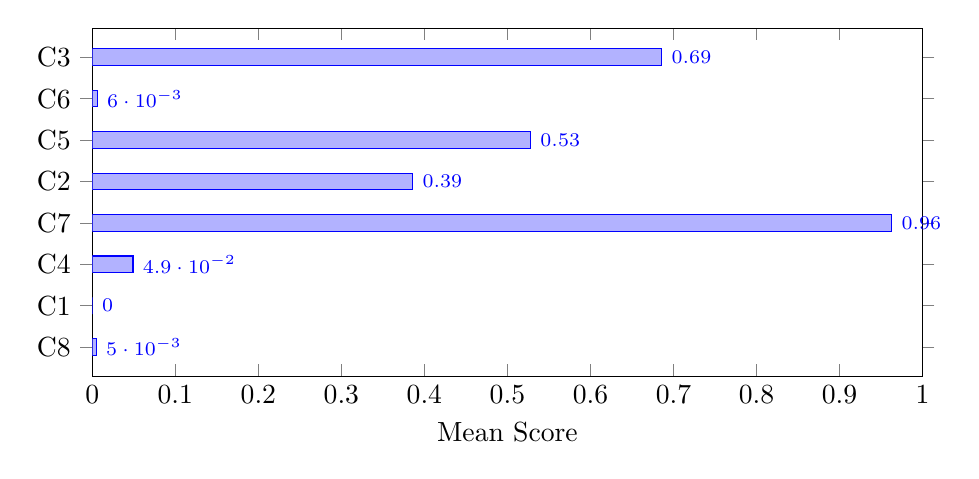
\begin{tikzpicture}
\begin{axis}[
    xbar,
    width=\columnwidth,
    height=6cm,
    xlabel={Mean Score},
    symbolic y coords={C8,C1,C4,C7,C2,C5,C6,C3},
    ytick=data,
    xmin=0,
    xmax=1.0,
    bar width=6pt,
    nodes near coords,
    every node near coord/.style={font=\scriptsize},
]
\addplot coordinates {
    (0.005,C8)
    (0.000,C1)
    (0.049,C4)
    (0.963,C7)
    (0.386,C2)
    (0.528,C5)
    (0.006,C6)
    (0.686,C3)
};
\end{axis}
\end{tikzpicture}
\caption{Measured mean criterion scores across 102 scenarios (seed = 42).
C7 saturates near 1.0 (shared residue accumulation) and C1 is constant
at zero in suite runs; C3 has the largest score variance and dominates
the composite ($\rho = 0.944$).}
\label{fig:criterion_contrib}
\end{figure}

\subsection{Baseline Comparisons}
\label{sec:baseline_results}

As shown in Table~\ref{tab:baselines}, AXIOM-02's action choice matches
the documented human expected action in 66.7\% of scenarios, vs 33.3\%
for the argmax baseline and 28.4\% for random selection (chance
$\approx 24.4\%$ given a mean of 4.09 actions per scenario). The
argmax strategy fails on moral-dilemma scenarios. We do not report a
single-drive baseline because it is not implemented in the released code.

% ============================================================================
\section{Discussion}
\label{sec:discussion}

\subsection{The Inhibition-Deliberation Thesis}
\label{sec:inhibition_thesis}

Our central claim is that mutual inhibition---rather than additive
activation---is the architectural feature that produces deliberative
signatures. When drives suppress each other asymmetrically, the system
can enter states where no drive dominates despite multiple drives being
highly activated. This produces deadlock, which in turn produces the
oscillation, hesitation, and spite signals that are read as
structurally analogous to human moral struggle.

The matrix $\mathbf{I}$ is not arbitrary: it encodes psychologically
grounded relationships (rage inhibits fear via adrenaline override; love
inhibits revenge via empathic interference). This means that the
network's dynamics are structured similarly to competitive
architectures in computational emotion models \citep{ledoux1996,
panskepp2004}.

\subsection{Spite as Non-Instrumentality}
\label{sec:spite}

The spite index (C6) is a measurement of one claimed phenomenon
invisible to conventional reward-maximising agents: choosing harm to
oneself specifically to assert autonomy. Dostoevsky's Underground Man
\citep{dostoevsky1864} is the canonical image of it. In AXIOM-02, the
detector fires when a weighted emotional charge, computed from the
effective activations of resentment, rage, and pride with per-drive
weights, exceeds a threshold ($\tau_{\text{spite}} = 0.58$); the cold
(rational) option is available but *not* chosen; and the chosen action
inflicts net harm on the subject beyond a floor
($\tau_{\text{harm}} = 0.25$) relative to the cold baseline.

\subsection{Moral Residue and Path-Dependent Character}
\label{sec:residue}

The moral-residue tracker (C7) implements what we call \emph{path-dependent
character}: prior decisions leave a guilt/shame/grief trace that modifies
future responses. This is not mere hysteresis; the residue is selective.
A system that yielded its organ in B01 shows amplified betrayal rage in
B02---because the sacrifice was not abstract but directed at the specific
person who later betrayed it.

This mechanism produces the literary phenomenon of character arc: Valjean's
mercy toward Javert in Les Mis\'{e}rables \citep{hugo1862} is only
explicable if we understand his prior history of reform. The moral residue
tracker makes such path-dependence explicit and measurable.

\subsection{Limitations}
\label{sec:limitations}

Several limitations warrant discussion. First, the scenario corpus is
drawn from Western literary canonical works, introducing cultural bias.
Second, the 20-step simulation window may truncate deliberation in
scenarios requiring longer temporal horizons. Third, the deliberative
criteria, while empirically motivated, have not been validated against
independent human judgements. Fourth, the epigenetic sensitivity
modification is currently limited to a small set of event types; a
more general learning rule would improve character formation dynamics.
Fifth, the deliberative complexity metric measures behavioural richness
in moral deliberation rather than consciousness per se; future work
should establish whether high $\DCI$ scores correlate with subjective
experience or whether they capture a structurally analogous but
ontologically distinct property.

% ============================================================================
\section{Conclusion}
\label{sec:conclusion}

We have presented AXIOM-02, a deterministic simulation engine that models
deliberative behaviour through mutual inhibition of affective drives. The
system produces measurable behavioural signatures---deadlock, oscillation,
spite-driven choices, and moral-residue bleed---and its action choice
matches the documented human expected action in 66.7\% of 102 literary
scenarios (seed = 42), versus 33.3\% for argmax and 28.4\% for random
selection (chance $\approx 24\%$). The composite metric $\DCI$ itself is
dominated by one binary criterion (C3, $\rho = 0.944$) and is reported
here as a diagnostic, not as a validated measure of deliberative
complexity. Human-validational claims are deliberately withheld: no
independent human judgements have yet been collected (see
Section~\ref{sec:limitations}).

The inhibition-deliberation hypothesis---that inter-drive suppression,
rather than additive activation, drives believably conflicted
decisions---remains the motivating architecture, supported at present
only by the measured fidelity effect of the full drive network over
baselines. Future work will: (1) run the validation framework with
independent raters; (2) per-chain-scope the residue tracker so C7 and
C1 score per scenario; (3) extend the scenario corpus; and (4) publish
the $\tau_f/\tau_s$ grid from the measurement harness.

\bibliographystyle{plainnat}
\bibliography{references}

\end{document}
